\documentclass[conference,a4paper]{../../sty/IEEEtran}

\usepackage{graphicx}

% *** GRAPHICS RELATED PACKAGES ***
\ifCLASSINFOpdf
  % \usepackage[pdftex]{graphicx}
  % declare the path(s) where your graphic files are
  % \graphicspath{{../pdf/}{../jpeg/}}
  % and their extensions so you won't have to specify these with
  % every instance of \includegraphics
  % \DeclareGraphicsExtensions{.pdf,.jpeg,.png}
\else
  % or other class option (dvipsone, dvipdf, if not using dvips). graphicx
  % will default to the driver specified in the system graphics.cfg if no
  % driver is specified.
  % \usepackage[dvips]{graphicx}
  % declare the path(s) where your graphic files are
  % \graphicspath{{../eps/}}
  % and their extensions so you won't have to specify these with
  % every instance of \includegraphics
  % \DeclareGraphicsExtensions{.eps}
\fi


% *** MATH PACKAGES ***
%\usepackage[cmex10]{amsmath}


% *** SPECIALIZED LIST PACKAGES ***
%\usepackage{algorithmic}


% *** ALIGNMENT PACKAGES ***
%\usepackage{array}


% *** SUBFIGURE PACKAGES ***
%\usepackage[tight,footnotesize]{subfigure}
%\usepackage[caption=false]{caption}
%\usepackage[font=footnotesize]{subfig}


% *** PDF, URL AND HYPERLINK PACKAGES ***
%\usepackage{url}


% *** Do not adjust lengths that control margins, column widths, etc. ***
% *** Do not use packages that alter fonts (such as pslatex).         ***
% There should be no need to do such things with IEEEtran.cls V1.6 and later.
% (Unless specifically asked to do so by the journal or conference you plan
% to submit to, of course. )


% correct bad hyphenation here
\hyphenation{op-tical net-works semi-conduc-tor}


\begin{document}
%
% paper title
% can use linebreaks \\ within to get better formatting as desired
\title{Bluetooth Low Energy Positioning}


% author names and affiliations
% use a multiple column layout for up to three different
% affiliations
\author{
\IEEEauthorblockN{Zhen-Huan Hwang and Hasan Mahmood Aminul Islam}
\IEEEauthorblockA{Aalto University, Espoo, Finland\\
zhen-huan.hwang and hasan.islam @aalto.fi}}


% make the title area
\maketitle


\begin{abstract}

Arduino is an open-source physical computing platform based on a simple i/o board and a development environment that implements the Processing/Wiring language. In this article, we will present a prototype of indoor positioning system using Arduino device and BLE shield which is designed to work with Arduino boards, including Arduino Uno, Mega 2560, Leonardo and Due. It allows us to connect Arduino board with other BLE Central device like a smartphone or tablet. 

\end{abstract}
% IEEEtran.cls defaults to using nonbold math in the Abstract.
% This preserves the distinction between vectors and scalars. However,
% if the conference you are submitting to favors bold math in the abstract,
% then you can use LaTeX's standard command \boldmath at the very start
% of the abstract to achieve this. Many IEEE journals/conferences frown on
% math in the abstract anyway.

% no keywords



\section{Introduction}
% no \IEEEPARstart
Arduino is an open-source physical computing platform based on a simple i/o board and a development environment that implements the Processing/Wiring language. Arduino can be used to develop stand-alone interactive objects or can be connected to software on your computer (e.g. Flash, Processing, MaxMSP). BLE Shield stands for Bluetooth Low Energy (BLE) Shield that is designed to work with Arduino boards, including Arduino Uno, Mega 2560, Leonardo and Due. It allows us to connect Arduino board with other BLE Central device like a smartphone or tablet. Android 4.3 (API Level 18) introduces built-in platform support for Bluetooth Low Energy in the central role and provides APIs that apps can use to discover devices, query for services, and read/write characteristics.



% Note that IEEE does not put floats in the very first column - or typically
% anywhere on the first page for that matter. Also, in-text middle ("here")
% positioning is not used. Most IEEE journals/conferences use top floats
% exclusively. Note that, LaTeX2e, unlike IEEE journals/conferences, places
% footnotes above bottom floats. This can be corrected via the \fnbelowfloat
% command of the stfloats package.
\section{Algorithm}



\begin{equation}
  RSSI = -(10n \log_{10}d + A)
\end{equation}

where, n,d and A are signal propagation constant, distance from sender and received signal strength at 1 meter distance


\section{Experimentation Setup}

\begin{figure}[h!]
\centering
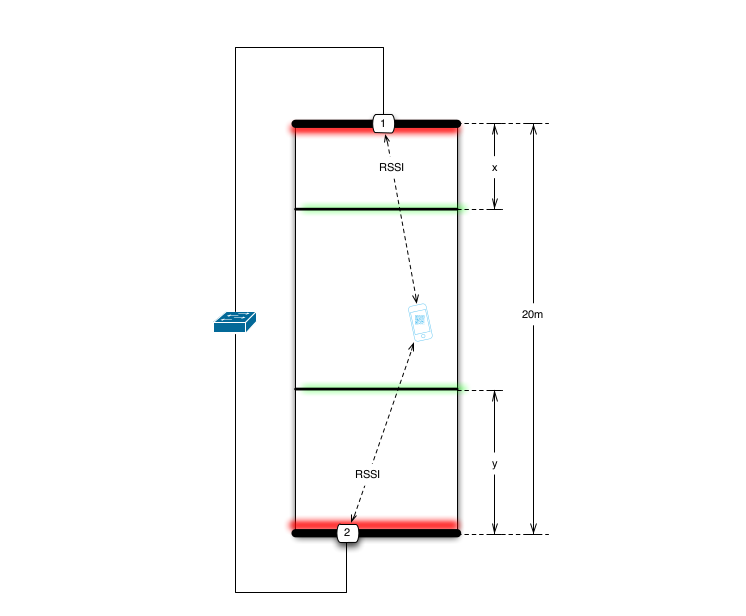
\includegraphics[scale=0.5]{position.png}  
\caption{Experimental Setup}
\label{fig1}


\end{figure}

\section{Result}

\section{Analysis}


\section{Conclusion}
The conclusion goes here.



% conference papers do not normally have an appendix


% use section* for acknowledgement
\section*{Acknowledgment}


The authors would like to thank...




% trigger a \newpage just before the given reference
% number - used to balance the columns on the last page
% adjust value as needed - may need to be readjusted if
% the document is modified later
%\IEEEtriggeratref{8}
% The "triggered" command can be changed if desired:
%\IEEEtriggercmd{\enlargethispage{-5in}}

% references section

\bibliographystyle{../../sty/IEEEtran}
\bibliography{ble}


\end{document}

